At the end of section~\ref{chp:SOLO_Quite_time}, \citet{Mason-2021-SolOQuietTime} reported the radial gradient of \ac{ACR} oxygen and helium-4 with energies of 4.4 MeV/nuc within 1 au. The analysis was based on the measurements from the \ac{SIS} instrument in 2020, and particle intensities were plotted as a function of three radial locations. Due to limited counting numbers, the flux uncertainties of flux were relatively significant. However, the results still indicate a positive and small gradient for oxygen compared to the observations from Helios and \ac{PSP} \citep{Marquardt2018AA,Rankin2021ApJ}.

As of 2023, the changing solar activity and the solar modulations have also influenced \acp{ACR} in the inner heliosphere as they propagate inward and diffuse throughout the heliosphere. Those changes are reflected in the variation of \ac{ACR} intensities and potentially in that of the radial gradient.
Meanwhile, the \ac{SolO} has completed its fifth orbit and continues its journey in the inner heliosphere. The \ac{HET} on board \ac{SolO}, which has been measuring helium of tens of MeV/nuc during the last two years, witnessed the change of solar activity and solar modulation.

Therefore, in this chapter, we investigate new \ac{ACR} observations in the inner heliosphere and in the new solar cycle, utilizing new data from \ac{HET} on board \ac{SolO}. We present the spectra and radial gradient of \ac{ACR} helium in the inner heliosphere between 2020 and 2022, taking into account possible interruptions such as \acp{SEP}, periodically occurring \acp{CIR} and long-term solar modulation.
Preliminary results indicate the consistent helium measurements of \ac{HET} and other instruments, for example, the \ac{SOHO}/\ac{EPHIN}. The radial gradients of helium-4 agree well within the large uncertainties with previous results from \ac{PSP}. The variation of the helium radial gradient in the early phase of solar cycle 25 is also discussed.

The details of the data analysis and results are given below. It is worth noting that results have not yet been published. We plan to continue this analysis and prepare a final publication to be submitted to Astronomy and Astrophysics soon.


\section{Introduction}

\acp{ACR} are accelerated interstellar pick-up ions characterized by the abundance of singly ionized atomic nuclei widespread in the heliosphere and predominant in the energy range of tens of MeV/nuc. They originate from the interstellar neutral particles, which are ionized by the solar wind via the charge exchange process when they flow into the heliosphere. Once they become ionized, the solar wind carries these charged particles to the outer heliosphere, where particles gain energy.
One source of \acp{ACR} is believed to be the blunt termination shock located at the boundary of heliosphere \citep{McComas2006GeoRL}. Since the \acp{ACR} ware first discovered in 1970, scientists have confirmed the observations of \ac{ACR} helium, oxygen, neon, and also protons in the outer heliosphere \citep{Garcia1973ICRC,Hoverstadt1973PhRvL,McDonald1974ApJ,Potgieter2013LRSP}.

Generally, the transport of the cosmic rays in the heliosphere are described by the interaction between charged particles and the interplanetary magnetic field embedded in the solar wind. The different physical processes that affect the propagation of particles are (a) diffusion caused by the irregular magnetic field, (b) adabitic energy loss and convection due to the expanding solar wind, and (c) gradient and curvature drifts in the heliospheric magnetic field.
Though the cosmic ray transport equations describe and model those basic processes \citep{Parker1965Pss,Jokipii1977ApJ,Jokipii1981ApJ,McDonald2001ICRC} in general, the detailed roles of each component interacting with the varying solar magnetic field in the inner heliosphere. i.e., within 1 au, still need to be fully understood. New measurements by \ac{PSP} indicate that the radial gradient of the lower energy cosmic rays within 1 au is inconsistent with the model prediction \citep{Rankin2021ApJ}.

The spatial gradients, including both radial and latitudinal gradients, provide valuable insights into the variation of drift effects of charged particles during the different solar cycles. As elucidated by \citet{Jokipii1977ApJ, Jokipii1979ApJ, Potgieter2013LRSP}, the drift direction of energetic particles differs with the polarity of the Sun's magnetic field, which alternates approximately every 11 years and results in the formation of a 22-year variation. The recent solar activity minimum in 2020 denotes positive polarity (A+). Consequently, the positively charged ions drift inward from the south and north pole regions while moving outward along the equatorial plane through the current sheet. Conversely, during the opposite polarity (A-) period, ions drift inward from the equator and exit through the poles. The drift direction of electrons is opposite to that of ions. These drift effects are manifested in spatial gradients. Previous observations from the Voyager and the Pioneer missions have indicated that the latitudinal gradient changes sign between two consecutive solar cycles belonging to different polarities, in agreement with predictions from transport models \citep{Mckibben1979ApJ, Cummings1987GeoRL, Christon1986JGR}. Moreover, the magnitude of the radial gradient varies between between different solar cycles of opposite polarity \citep{Rankin2021ApJ,Rankin2022ApJ,Giacalone2022SSRv,Webber1981JGR,Marsden1999AdSpR}.

%Despite of this, the precious radial gradient of the current solar cycle especially during the ininial phase of the new solar cycle are not measured and determined.
According to \citet{Rankin2021ApJ}, the radial gradient of cosmic rays can be expressed as:
\begin{equation}
    g_r = \frac{1}{f}\frac{\partial{f}}{\partial{r}} = \frac{\partial{\mathrm{ln} f}}{\partial{r}} \enspace ,
    \label{eq:radial_gradient}
\end{equation}
where $g_r$ denotes the differential radial gradient component under the assumption that the latitude gradient is negligible. The gradient represents the change of the differential flux, $f$ with respect to radial distance $r$. The radial gradient can be obtained by fitting the data to a linear equation using the least square method.


Benefiting from its unique orbits, which have the closest perihelion distance of 0.28 au, \ac{SolO}, launched on Feb 10, 2020, have provided valuable measurements of cosmic rays during the quiet time, shedding light into the transport effects of cosmic rays in the inner heliosphere by deriving the radial gradient of those particles.
In Fig.~\ref{fig:SOLO_orbit_info}, we present the orbit information of \ac{SolO} from Feb 2020 to May 2023. The top three panels display the radial distance of \ac{SolO} to the Sun, Carrington longitude, and Carrington latitude of \ac{SolO}. As depicted in the top panel, \ac{SolO} has completed five orbits and is moving away from the Sun after passing its sixth perihelion. The closest distance to the Sun was achieved during the fifth orbit in September of 2022. 
The Carrington longitude of \ac{SolO} indicates its movement relative to a fixed longitude line on the Sun. Originally defined from Earth's perspective, with a mean synodic period of approximately 27.2753 days, the Carrington system and its origin point are applied to the \ac{SolO} coordinate system. 
Due to the greatly varying radius of the orbit, orbital periods of \ac{SolO} Carrington rotations range between 26.6 and 35.8 days, slightly differing from the period of Earth. Currently, the latitude of \ac{SolO} is constrained within a range of $\sim$ $\pm$8 degrees.
In addition, we provide the radial distance and the longitudinal separation between \ac{SolO} and Earth to illustrate the relative positions.

To better visualize and understand \ac{SolO}'s movement in the inner heliosphere and its relation to the Sun and Earth, we depict the orbit track of \ac{SolO} in two coordinate systems in Fig.~\ref{fig:SOLO_orbit_track}. The top panel shows the orbit in the heliocentric coordinate system, where the mean equinox is used as the reference direction of x-axis. In this coordinate system, \ac{SolO}'s orbit exhibits an elliptical shape. Similarly, the bottom panel of Fig.~\ref{fig:SOLO_orbit_track} presents the trajectory in a heliographic coordinate system, with the Sun fixed in the center and the Earth positioned at 1 au, marked as the blue dot. The x-axis is aligned to the Sun - Earth direction. In this coordinate system, orbits appear twisted and undergo changes in shape.

The color bars in both panels indicate the time sequence from February 2020 to May 2023. The numbers of Carrington rotations are marked at the beginning of each rotation and labeled next to the orbit track. The moving direction of the spacecraft can be inferred from changes in the numbers and colors.
%Obviously, when the spacecraft is located away the sun, the \ac{SolO} is moving in a limited region, with hardly changed longitude in one Carrington rotation. Conversely, the longitudinal changes are large when \ac{SolO} rapidly passes by the sun. Between them, the radial distance changes quickly. 


%In this report, we organized the content as follows: We first introduce the data and instrument we used in this work, which including the SOLO/HET, SOHO/EPHIN, STEREO/LET and possiblely LND. In chapter 3 we give the overview of the observation of the helium-4 between 2020 and 2022 when in the second half, SEPs frequently happens and the overall cross-calibration between different instrument

%In section4, we explain the several kind of effect that could disturbe the constanct background and show how the result are affected by different method. In the end, we conclude.



\begin{figure}
    \centering
    \includegraphics[width = \textwidth]{images/ACR/SOLO_orbit_helioscentric_3.png}
    \caption[The orbit variation of \ac{SolO} in Carrington coordinate system]{(From top to bottom) The variation of \ac{SolO}'s radial distance, Carrington longitude, Carrington latitude as well as the distance and longitude separation between \ac{SolO} and \ac{SOHO}. The period covered in the figure ranges from February 2020 to May 2023. }
    \label{fig:SOLO_orbit_info}
\end{figure}
\begin{figure}
    \centering
    \includegraphics[width=0.8\textwidth]{images/ACR/SOLO_orbit_track_helioscentric_3.png}
    \includegraphics[width = 0.8\textwidth]{images/ACR/SOLO_orbit_stonyhurst_3.png}
    \caption[Orbit track of \ac{SolO}]{Top: The orbit track of \ac{SolO} in the heliocentric mean ecliptic coordinate system where the origin is the center of the Sun, and x-axis points to the mean equinox and the xy - plane is the ecliptic plane. Bottom: The orbit track of \ac{SolO} in the Stonyhurst coordinate system. Earth is fixed at 1 au and is marked with a solid blue circle. The other measurements from \acs{SOHO}/\acs{EPHIN}, \acs{ACE}/\acs{CRIS}/\acs{ACESIS} and \acs{LND} are from locations near Earth. The numbers next to the dashed circle lines indicate the distance from the Sun to 1 au.
    The blue dots along the track indicate the start of each Carrington rotation of \ac{SolO}. About 37 Carrington rotations are used in this study, as the numbers next to the tracks show. The period ranges from February 2020 to May 2023.}
    \label{fig:SOLO_orbit_track}
\end{figure}




\section{Instruments and data employed in this study}


The charged particle measurements reported in this study are from \ac{HET} onboard \ac{SolO}, which could measure charged particles in the energy range from tens of MeV/nuc to a hundred MeV/nuc. Specifically, we focus on helium particles within the energy range of 10 - 50 MeV/nuc, which are the \ac{HET} stopping particles measured in detector C. During quiet times, the predominant particles are \acp{ACR} in this energy range. Further details regarding the \ac{HET} measurement principle can be found in section \ref{sec:Solar_Orbiter} and \citet{RodriguezPacheco-2019-EPD}.

Similar to the analysis by \citet{Mason-2021-SolOQuietTime} for \ac{SIS}, our analysis of the helium radial gradients measured by \ac{HET} is also constrained by the counting statistics due to the limited geometry factor of \ac{HET} and the low helium intensities in space. In order to derive radial gradients with better accuracy, we employ two methods to increase count statistics and hence reduce uncertainties of gradients. In the first method, we calculate a summation of count rates measured by four \ac{HET} apertures. There are two sets of \ac{EPT}/\ac{HET} telescopes mounted perpendicularly on the \ac{SolO}, with each measuring stopping particles from two ends. Hence, \ac{SolO}/\ac{HET} can provide helium flux measurements from sunward, anti-sunward, southward, and northward directions. In the following analysis, we simply use the averaged helium intensity from four directions as the measurement of \ac{SolO}. By doing so, we can reduce the uncertainties of helium intensity to half. Secondly, we rebinned the fine energy channels of \ac{HET} and reconstructed four energy channels in the energy range of 11.1 - 19.4 MeV/nuc, 19.4 - 29.5 Mev/nuc, 29.5 - 41.2 Mev/nuc, 41.2 - 49.0 Mev/nuc, to further increase the counting statistic of each channel.



In addition to the nominal data products, designed for scientific purposes and measuring the flux of different charged particles of different energies, we also take advantage of one type of housekeeping data as an indicator of \ac{SEP} events. This housekeeping data registers every particle that can trigger two \acp{SSD} (A and B) in coincidence but without resolving the particle species and their primary energies. This counter also has a larger \ac{FOV}. Therefore, it has more significant counting statistics than the nominal scientific data products, which can better determine the onset and the end of the \ac{SEP} events. In Fig.~\ref{Fig:solo-lvl2}, we present the hourly count rate of two multiple detector counters. One is from the sunward telescope, named HET\_any (a1,b1i), and the other is from the anti-sunward telescope, named HET\_any(a2,b2i). Later in Sec.~\ref{sec:sep_list_acr}, we explain how to use these counters to filter the \ac{SEP} events.


%This trigger can detect energetic electrons, protons, and heavy ions without any element resolution, 
%The periods are determined by the 3-sigma method \citep{Xu2017ApJ,Xu2020ApJ, Huttunen2005AA}, which is commonly used in determining the onset time of the \ac{SEP} event. In this method, if intensities of data points are about 3 times the standard deviation higher than the background intensity, these data points are defined as the \ac{SEP}.

Apart from \ac{HET}, we also used the observations from instruments or spacecraft close to Earth for comparison. We use helium and heavy ion measurements from the \ac{ACESIS} and the \acl{CRIS}\ac{CRIS} onboard the \ac{ACE}, helium measured by \acl{SOHO}/\acl{EPHIN} and helium intensity measured by \acl{LND}\acused{LND} on the lunar far-side surface. \ac{STEREOLET} provides helium measurements with energy below 10 MeV/nuc from the \ac{STEREO}-A spacecraft. But only \ac{SOHO}/\ac{EPHIN} is used as the baseline of the long-term trend of helium-4 anomalous cosmic rays.

\section{Overview of observations between 2020 and 2022 and the cross-calibration between four instruments}

\subsubsection*{Comparison of spectra between \ac{HET} and other instruments}
%\addtocontents{toc}{\protect\setcounter{tocdepth}{1}}
%%%%%% review to here.
Before deriving radial gradients of helium, it is necessary to provide an overview of the \ac{HET} observations of heavier ions, such as helium, carbon, nitrogen, and oxygen. Fig.~\ref{fig:overview} illustrates the averaged spectra between 2020 and 2022 after removing possible \ac{SEP} periods.


The \ac{HET} measurements are represented by diamonds of various colors, with red for helium-4, orange for carbon, green for nitrogen, and blue for oxygen.
The helium spectrum spans a wide energy range and consists of particles stopping in detector B ($<$ 10 MeV/nuc), stopping in detector C (10 - 100 MeV/nuc), and penetrating particles ($>$ 100 MeV/nuc). 
The analysis of \ac{ACR} helium radial gradients is based only on measurements of helium-4 stopping in detector C.
%e penetrating helium comprises two populations depending on their primary energy: the barely penetrating helium marked as empty red diamonds and the fully penetrating particle with energy above 200 MeV/nuc. 
%%% here  ----
Although they are not used in this study, it is worth noting that the intensities measured by two channels around 100 MeV/nuc are a few times higher than those in the nearby channels. The reason for these abnormal increases is yet unknown.
%probably due to the dead layer before each detector \citep{Wimmer2021AA}. It also possible that the energy channels have not been properly calibrated.
Besides, when converting counts to fluxes in the \ac{GCR} spectrum, geometry factors of fully penetrating particle channels, i.e., the last three channels, are calculated based on the 4$\pi$ simulation. That is because \ac{HET} could not distinguish incident directions of those fully penetrating particles, which are mainly \acs{GCR}. Unlike \acs{SEP}, \acs{GCR} are nearly isotropic in the heliosphere.

In Fig.~\ref{fig:overview}, \ac{ACE} measurements are plotted as circles, including filled circles representing \ac{ACESIS} and empty ones for \ac{CRIS}. Unfortunately, at the moment, helium measurements from \ac{ACE} are available only below 15 MeV/nuc. Hence, we use helium data from \ac{SOHO}/\ac{EPHIN} which are shown as purple squares, to calculate radial gradients of \ac{ACR} helium. Besides, \ac{LND}-measured helium-4 is also shown as brown triangles. \ac{EPHIN} covers the \ac{ACR} energy range of 10 - 50 MeV/nuc while \ac{LND} covers the energy range of 10 - 35 MeV/nuc.

Fig.~\ref{fig:overview} reveals a general agreement of the averaged spectra of four particle species, though measurements come from different instruments and distinct positions. Furthermore, the flat helium spectra between 10 MeV - 50 MeV/nuc and the peak intensity of oxygen and nitrogen at 10 MeV/nuc demonstrate the presence of the \ac{ACR} components in the inner heliosphere. 

Fig.~\ref{fig:helium_spec_1au} focuses on the helium-4 spectra based on the measurements when \ac{SolO} was positioned between 0.95 and 1 au, after subtracting measurements of \acs{SEP}. The periods when \ac{SolO} was close to 1 au in the last two years are given in Tabel \ref{tab:1AU_period}, which consists of start times, end times, and the relative distance from \ac{SolO} to Earth.
The averaged spectrum of \ac{EPHIN} and \ac{HET} helium at energies above 10 MeV/nuc are comparable. Therefore, we utilize the \ac{EPHIN} and \ac{HET} helium measurements within the energy range of 10 to 50 MeV/nuc in the subsequent analysis.
A discrepancy between the spectra appears in energy channels below 10 Mev/nuc where intensities of \ac{ACESIS} and \ac{HET} are about two times higher than those of \ac{EPHIN}. Besides, the \ac{LND} spectrum appears generally higher than the other measurements and has larger error bars. The more significant uncertainties are due to the limited operation time on the lunar surface (see section \ref{sec:change_4_LND}). The spectra don't agree for quiet times, which may be due to different background levels of the instruments.





\begin{figure}[!htb]
    \centering
    \includegraphics[width = 0.8\textwidth]{images/ACR/ACE_SIS_CRIS_SOLO_all_3.png}
    \caption[The quiet time spectra of helium, carbon, nitrogen, and oxygen between 2020 and 2022]{The helium-4 (red, brown, purple), carbon (orange), nitrogen (green), and oxygen (blue) spectra averaged between 2020 and 2022. \ac{SEP} events have been removed. The data used in this figure covers observations from \ac{SolO}/\ac{HET}, \ac{SOHO}/\ac{EPHIN}, \ac{ACE}, and \ac{LND}.}
    \label{fig:overview}
\end{figure}
\begin{figure}[!htb]
    \centering
    \includegraphics[width = 0.8\textwidth]{images/ACR/1AU_comparison_ACE_EPHIN_SOLO_SEP_version2.png}
    \caption[The helium spectra when \ac{SolO} was between 0.95 and 1 au]{The helium-4 spectra of \ac{SolO}/\ac{HET}, \ac{SOHO}/\ac{EPHIN}, \ac{ACE}/\ac{ACESIS} and Chang'4/\ac{LND} when SOLO was between 0.95 and 1AU. \ac{SEP} events have been removed according to the \ac{SEP} list in Appendix \ref{Appendix:SEPlist}.}
    \label{fig:helium_spec_1au}
\end{figure}

\subsection*{Temporal variation of helium-4 intensity}


\begin{figure}[!htb]
    \centering
    \includegraphics[width = 0.8\textwidth]{images/ACR/overview_Helium_4_instrument.png}
    \caption[Overview of helium intensities measured by different instruments]{From top to the bottom: The daily averaged helium flux measured by \ac{SolO}/\ac{HET}, \ac{SOHO}/\ac{EPHIN}, Chang'E-4/\ac{LND}, and \ac{STEREO}-A/\ac{STEREOLET} over 2020.2 - 2022.10. The bottom plot shows the radial distance of \ac{SolO} from the Sun.}
    %The red dashed lines indicate the SEP events that we determined by eye.
    %\TODO{reminder: you should better re-load the SOLO data, and check the isotropic between different directions, and resample data before further process like sum all direction or somesome.}}
    \label{fig:overview_helium_intensity}
\end{figure}

Fig.~\ref{fig:overview_helium_intensity} presents intensity profiles of helium from February 2020 to October 2022 from \ac{HET}, \ac{EPHIN}, \ac{LND}, and \ac{STEREOLET}. The energy ranges of reconstructed channels are labeled in the corresponding legends. The bottom panel shows the distance of \ac{SolO} from the Sun.


Figure~\ref{fig:overview_helium_intensity} clearly shows that helium fluxes are relatively stable from 2020 to the middle of 2021, dominated by cosmic rays; only one large \ac{SEP} event occurred at the end of 2020 \citep{Kolhoff2021AA}. 
Since the second half of 2021, more \acp{SEP} have been observed and were measured by different instruments, for instance, \ac{HET} and \ac{EPHIN}, as shown in the top two panels of Fig.~\ref{fig:overview_helium_intensity}.
Those large and intense \acp{SEP} significantly disturb the time profile of the \ac{ACR} background and, consequently, must be removed before we calculate the \ac{ACR} radial gradient. 
Of note, the energetic helium arrives differently at \ac{SolO}, \ac{SOHO}, and \ac{STEREO}-A. The discontinuities of \ac{LND} measurements are due to the hibernation of \ac{LND} during the local night on the Moon's far-side surface.


In addition to the intermittently occurring \acp{SEP}, a long-term decrease is also clearly seen in the \ac{HET} and \ac{EPHIN} time profiles from 2020 to the end of 2022. This decrease is caused by the enhanced solar modulation, which significantly reduces the number of \acp{ACR} arriving at Earth and in the inner heliosphere within one astronomical unit. We expect a further decrease of the \ac{ACR} intensity in the next few years before the solar activity reaches its next maximum.

In contrast to the transient variation from \acp{SEP} and 11-year variation attributed to the large-scale solar modulation, the intensities of cosmic rays are additionally influenced and modulated by recurring, compressed structures that are formed by the interaction between fast and slow solar wind stream emitted from the solar corona. These compressed structures, known as stream interaction regions or corotating interaction regions, periodically enhance the pressure and density of the plasma and corotate with the Sun, aligned with the Sun's rotation \citep{Burlaga1974JGR, Gosling1976JGR, Richardson2004SSRv}. Those changes in local conditions modify the transport of cosmic rays, resulting in decreases of the intensity of the order of 1 - 5 \% \citep{Richardson2004SSRv, Richardson-2018}, which are not as significant as those induced by \acp{SEP} and overall solar modulations.

\begin{table}[!htb]
    \centering
    \caption[Time periods when \ac{SolO} closed to 1 au]{A list of time periods when \ac{SolO} is between 0.95 and 1 au. The distances between \ac{SolO} and Earth are also given.}
    \label{tab:1AU_period}
    \begin{tabular}{|c|c|c|c|}
    \hline
    number of period & start time & end time & distance to Earth  (au)\\
    \hline
    1   & 2020-02-28 & 2020-03-16   & 0.07 \\
    \hline
    2   & 2020-09-14 & 2020-11-10   & 1.76 \\
    \hline
    3   & 2021-05-27 & 2021-06-09   & 1.49 \\
    \hline
    4   & 2021-11-21 & 2022-01-15   & 0.13 \\
    \hline
    5   & 2022-06-05 & 2022-08-02   & 1.96 \\
    \hline
    6 (not used)    & 2023-01-04 & 2023-01-17   & 0.41 \\
    \hline
    \end{tabular}
\end{table}

\section{Averaged helium intensity profile between 2020 and 2022}
\subsection*{Solar energetic particle events list}
\label{sec:sep_list_acr}

As previously mentioned, \ac{SEP} events significantly disturb the \ac{ACR} background. Therefore, it is crucial to have a complete and properly defined list of \ac{SEP} periods. This section describes the methodology and data products we used to determine the \ac{SEP} periods. The \ac{SEP} lists are determined separately for \ac{SolO} and \ac{SOHO}/\ac{EPHIN} since \acp{SEP} arrived differently at \ac{SolO} and at Earth. 

To thoroughly remove \acp{SEP} and mitigate the presence of residual particles that may not be directly recognized from intensity profiles, we use different data products to identify \acp{SEP} rather than relying solely on helium data.

The multiple detector counters of \ac{HET} sunward and anti-sunward telescope are employed to determine \ac{SEP} observed by \ac{SolO}. As shown in Fig.~\ref{Fig:solo-lvl2}, the hourly counts of two counters range from approximately 600 to 800 during quiet time. When \ac{SEP} occurred, both counters increased significantly and exceeded the background, though the peak values of two counters might differ depending on the pitch angle distribution of \acp{SEP}. We use the sunward measurements to determine the \ac{SEP} periods. 
For \acp{SEP} reaching Earth, we utilize the time profile of protons in the energy range below 10 MeV observed by \ac{EPHIN} to determine \acp{SEP}. The corresponding proton profiles are displayed in Fig.~\ref{Fig:SOHO_EPHIN_Proton_flux}

The durations of \ac{SEP} events are determined using the 3-$\sigma$ method, supplemented by eye inspection. Here, $\sigma$ is the standard deviation of background measurements taken during pre-event quiet periods. \ac{SEP} periods are defined as consecutive time intervals when the flux exceeds three times the standard deviation above the background. This method is commonly used to determine the onset time of \ac{SEP} events and is valid for those \acp{SEP} with clear onset and sharp increase.

However, if the background is unclear and the increase of the temporal profiles is slow, the determination of the onset and end of the event might have a larger uncertainty. In this case, we check the results manually and determine the boundaries of the \ac{SEP} periods by eye. As a result, the \ac{SEP} periods that we determined are illustrated as the magenta-colored regions in Fig.~\ref{Fig:solo-lvl2} and Fig.~\ref{Fig:SOHO_EPHIN_Proton_flux}. The \ac{SEP} periods are listed in Table ~\ref{tab:solo_SEPlist} and Table \ref{tab:SOHO_SEP_list} in Appendix \ref{Appendix:SEPlist}.





\begin{figure}
    \centering
    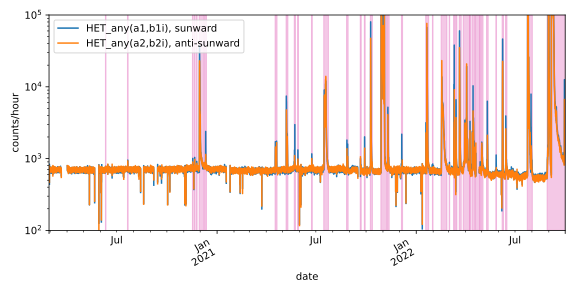
\includegraphics[width = \textwidth]{images/ACR/SOLO-lvl2-trriger-V2.png}
    \caption[The multiple detector counters of \ac{HET}]{Hourly count rate of the \ac{HET} multiple detector counters. The magenta-colored regions are the \ac{SEP} periods we identified.}
    \label{Fig:solo-lvl2}
\end{figure}



\begin{figure}
    \centering
    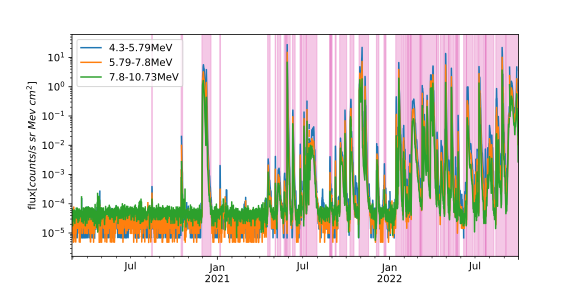
\includegraphics[width = \textwidth]{images/ACR/SOLO-EPHIN-l3i-log2+6-proton-6H-V2.png}
    \caption[The proton intensity profile observed by \ac{EPHIN}]{The proton flux measured by \ac{SOHO}/\ac{EPHIN} below 10 MeV. The data we used here are the level-3 proton data products generated from pha data \citep{kuehl2020JSWSC}. The magenta-colored regions indicate \acp{SEP} observed near Earth.}
    \label{Fig:SOHO_EPHIN_Proton_flux}
\end{figure}

\subsection*{Averaged over Carrington rotation}

As mentioned earlier, transient \acp{SEP}, long-term solar modulation, \acs{SIR}\acused{SIR} and quasi-periodic \acs{CIR} affect the \ac{ACR} intensity. In the previous section, we identified and removed \ac{SEP} periods to obtain a slowly changing profile. In this section, we will further reduce the impact of recurring compressed regions by averaging the intensity profile over each Carrington rotation, as suggested by \citet{Rankin2021ApJ}. One complete Carrington rotation corresponds to the period between two adjacent peaks of \ac{SolO}'s Carrington longitude, which is depicted in the second panel from the top of Fig.~\ref{fig:SOLO_orbit_info}.

%. Though that data point is from a Carrington rotation with a larger \ac{SEP} event, we have already removed the \ac{SEP} periods from the data. Besides, such an increase is even clearer in the higher energy channel (bottom panel). 

Fig.~\ref{fig:carrington_flux} displays the average helium flux from \ac{HET} (orange line) and \ac{EPHIN} (blue line) in four generally comparable energy bins though two different instruments from different locations measured them. Besides, both averaged fluxes decrease over time, which is noteworthy, indicating the largely increased solar modulation during the new solar cycle. The red dashed lines indicate the variation in radial distance between \ac{SolO} and the Sun. 

However, we could still see some discrepancies that are worth noting. During the end of 2020 and the start of 2021, the \ac{HET} helium intensity is unusually higher compared to that measured by \ac{EPHIN}. The discrepancies are up to 30 \% and are clearly seen in all four channels. Furthermore, the bottom panel of Fig.~\ref{fig:carrington_flux} shows that before 2021, the intensities of 38.5 - 53.0 MeV/nuc helium from \ac{EPHIN} are statistically lower than those from \ac{HET}. After that, such a discrepancy gradually disappeared in this channel. However, such a discrepancy is unseen in lower energy channels. Currently, the reasons for these discrepancies are unclear.

Fig.~\ref{fig:fluxvsdistance} illustrates the helium flux within the energy range of 11.1-19.4 MeV/nuc from \ac{HET}, shown as a function of the radial distance from 0.4 to 1 au. Data points of different colors represent the averaged fluxes during the Carrington rotation in different orbits, as indicated in the legends. The Carrington rotation numbers from 0 to 30 are also given. Notably, the intensity of helium at the last measurement point is about five times less than that at the beginning. Such a decrease is caused by the solar modulation. Removing this trend is discussed in the next section.

%Without carefully tackling this underlying baseline trend, we could not derive the radial gradient with a magnitude of $\sim$ 25\%/au.


% and the slight discrepancy in energy channels between \ac{HET} and \ac{EPHIN},

\begin{figure}
    \centering
    \includegraphics[width = 0.8\textwidth, height = 0.4\textwidth]{images/ACR/seperate_mask_1-3_newSOHOSEPmask/Carrington_SOLO_11.1-19.4MeV_EPHIN_10.7-20.3MeV.png}
    \includegraphics[width = 0.8\textwidth,height = 0.4\textwidth]{images/ACR/seperate_mask_1-3_newSOHOSEPmask/Carrington_SOLO_19.4-29.5MeV_EPHIN_20.3-28.0MeV.png}
    \includegraphics[width = 0.8\textwidth,height = 0.4\textwidth]{images/ACR/seperate_mask_1-3_newSOHOSEPmask/Carrington_SOLO_29.5-41.2MeV_EPHIN_28.0-38.5MeV.png}
    \includegraphics[width = 0.8\textwidth,height = 0.4\textwidth]{images/ACR/seperate_mask_1-3_newSOHOSEPmask/Carrington_SOLO_41.2-49.0MeV_EPHIN_38.5-53.0MeV.png}
    \caption[The averaged helium flux in four energy channels between 10 and 50 MeV/nuc]{The flux of \ac{SolO} (orange) and \ac{EPHIN} (blue) averaged over the Carrington rotation periods in the energy channels of 10 - 20 MeV/nuc, 20 - 30 MeV/nuc, 30 - 40 MeV/nuc, and 40 - 50 MeV/nuc. The daily averaged \ac{HET} helium fluxes are also shown in different energy channels as light orange lines. Red dashed lines are the radial distance of \ac{SolO} to the Sun.}
    \label{fig:carrington_flux}
\end{figure}

\begin{figure}
    \centering
    \includegraphics[scale = 0.8]{images/ACR/SOLO-flux_only.png}
    \caption[11.1 - 19.4 MeV/nuc \ac{HET} helium flux vs the radial distance of \ac{SolO}]{The change of flux of 11.1 - 19.4 MeV/nuc helium from \ac{HET} with respect to the radial distance of \ac{SolO}. The data for different orbits are presented in distinct colors. The numbers over data points indicate the order of time. }
    \label{fig:fluxvsdistance}  
\end{figure}


\section{Radial gradient of ACR helium}

Deriving the slight radial gradient ( $\sim$ 25\%/au, \citet{Rankin2021ApJ}) from the substantially changed data is challenging, specifically when dealing with the five-fold decrease in helium intensity resulting from solar modulation.
To address this challenge and obtain the radial gradient, we detrend the \ac{HET} flux by using the \ac{EPHIN} flux as a baseline. We assume that the solar modulation is the same for both instruments. We first calculate the ratio of \ac{HET} and \ac{EPHIN} and then estimate the radial gradient of different energy \ac{ACR} helium using the definition in Eq.~\ref{eq:radial_gradient}.

We present the temporal variation of flux ratio between \ac{HET} and \ac{EPHIN} for four energy channels in the first and third rows of Fig.~\ref{fig:ratio_radialgradient}. The various colored regions represent periods of different orbits. The second and fourth rows illustrate the ratio in log scale as a function of the radial distance. Here, only the data points from the first three orbits are shown and fitted. That is because \acp{SEP} are the dominant particles in the fourth orbit. Hence, most of the data are removed, causing considerably higher uncertainties in the result. The colored dashed lines in the figure represent the fitting results obtained for different orbits. The shaded regions surrounding these lines are the corresponding 95\% confidence intervals,  indicating the uncertainty of the fitting results. The averaged radial gradients of the first three orbits are depicted as black dashed lines, indicating the overall trend between 2020 and 2022.
In addition, we have summarized the radial gradient of \ac{ACR} helium in different energy channels and for different orbits in Table~\ref{Tab:radialgradient_1}.

\begin{figure}[!htb]
    \centering
    \includegraphics[width =0.48\textwidth, height = 0.48\textwidth]{images/ACR/seperate_mask_1-3_newSOHOSEPmask/ratio_time_radialgradient_10-20MeV_2.png}
    \includegraphics[width =0.48\textwidth, height = 0.48\textwidth]{images/ACR/seperate_mask_1-3_newSOHOSEPmask/ratio_time_radialgradient_20-30MeV_2.png}
    \includegraphics[width =0.48\textwidth, height = 0.48\textwidth]{images/ACR/seperate_mask_1-3_newSOHOSEPmask/ratio_time_radialgradient_30-40MeV_2.png}
    \includegraphics[width =0.48\textwidth, height = 0.48\textwidth]{images/ACR/seperate_mask_1-3_newSOHOSEPmask/ratio_time_radialgradient_40-50MeV_2.png}
    \caption[Ratio of helium intensity between \ac{HET} and \ac{EPHIN} and helium radial gradient in different energy range]{Row 1 and 3: The temporal variation of the helium flux ratio between \ac{HET} and \ac{EPHIN} measurements (averaged over their own Carrington rotation and interpolated to calculate the ratio) for different energies; Row 2 and 4: Flux ratio vs radial gradients in the first three orbits, overlay by the log-linear fitting lines.} 
    \label{fig:ratio_radialgradient}
\end{figure}



\begin{figure}[!htb]
    \centering
    \includegraphics[scale = 0.8]{images/ACR/Energydependent_normal_mask20230612.png}
    \caption[Energy dependency of the helium radial gradient]{The radial gradient of helium measured in the ecliptic plane at different energies. The values from \ac{HET} are given as orange diamonds with corresponding error bars. The multiple blue circles in the figure represent the gradient obtained from \ac{PSP} \citep{Rankin2021ApJ}.}
    \label{fig:comparison_SOLO_PSP}
\end{figure}

%  \TODO{New simulation and ask help from some one in Kiel, not now}.



\begin{table}[!htb]
    \centering
    \begin{tabular}{|c|c|c|c|c|c|}
        \hline
    Number of Orbit     & 1               & 2              & 3               & 4  & ave(1-3)\\
    \hline
                        &20200228 -      & 20201012-        & 20210602-    &  20211216-   &\\  
    Energy (MeV/nuc)    & 20201012        &  20210602       & 20211216      &  20220704  & \\

    \hline
    10 - 20 &  27 $\pm$ 9 & 38 $\pm$ 14 & 21 $\pm$ 19 & -25 $\pm$ 22 & 28$\pm$ 8\\
    \hline
    20 - 30 &  19 $\pm$ 9 & 28 $\pm$ 20 & 11 $\pm$ 15 & 33 $\pm$ 16 & 19$\pm$ 08\\
    \hline
    30 - 40 &  5 $\pm$ 14 & 12 $\pm$ 14 & 37 $\pm$ 21 & 8 $\pm$ 21 & 10$\pm$ 11\\
    \hline
    40 - 50 &  5 $\pm$ 9 & 27 $\pm$ 21 & 58 $\pm$ 19 & 20 $\pm$ 18 & 21$\pm$ 11\\
    \hline
    \end{tabular}
    \caption[Table of helium radial gradient]{Radial gradient of helium (\%/au) in different energy channels at different orbits between 2020 and 2022.}
    \label{Tab:radialgradient_1}
\end{table}
\subsection*{Radial gradient of helium vs energy}

Fig.~\ref{fig:comparison_SOLO_PSP} displays the energy dependence of the radial gradient of \ac{ACR} helium measured by \ac{PSP} and \ac{SolO}. 
Despite the significant uncertainties, radial gradients of helium measured by \ac{SolO} averaged over the first three orbits are shown as orange diamonds. Except for helium in the energy range of 30 - 40 MeV/nuc, which has a lower average gradient of 10 $\pm$ 11 \% /au, we report radial gradients of 28$\pm$ 8 \%/au, 19$\pm$ 8 \%/au, and 21$\pm$ 11 \%/au for helium energies of 10 - 20 MeV/nuc, 20 - 30 MeV/nuc and 40 - 50 MeV/nuc respectively.
Such gradients are consistent with \ac{PSP}'s results within the uncertainties.
To compare with \ac{PSP} results derived by \citet{Rankin2021ApJ}, we replot helium radial gradients as the blue circles at their energy range. \ac{PSP} measurements are from 2018 to 2019 in the same solar activity minimum but earlier than \ac{SolO}. The averaged radial gradient of helium in the energy range of 4 - 45 MeVn/nuc is about 25$\pm$5 \%/au. 



\subsection*{The time variation of the radial gradient}

We also present the time variation of the helium radial gradients for different energy ranges from 10 - 50 MeV/nuc in Fig.~\ref{fig:radialgradient_time_variation}. The behaviors exhibited by the various energy channels are distinct, and the radial gradients show significant variations from 2020 to 2022, probably due to increased solar activity. Several intriguing features are observed in the time variation of the radial gradients, which are unexpected and hard to explain.

The peaks of radial gradients occur at different times for each energy channel. The highest radial gradient for the 10 - 20 Mev/nuc helium channel appears during the second orbit, while for the 30 - 50 Mev/nuc channels, the peaked gradients are observed in the subsequent orbit.

Furthermore, the sign of the radial gradient in the energy range of 10 - 20 MeV/nuc changes from positive to negative during the fourth orbit in 2022. This change could be attributed to the more considerable uncertainties introduced by \acp{SEP}. Because of the more frequently appeared \ac{SEP} in the fourth orbit, we might remove most of the data from \ac{EPHIN} measurements in one Carrington rotation; thus, the remaining days' measurements are likely not representative of the whole Carrington rotation. Consequently, the Carrington averaged \ac{EPHIN} flux in the fourth orbit exhibit more fluctuations than the previous periods. 
An alternative explanation for the observed sign change in the radial gradient could be attributed to the complex magnetic field structures in the inner heliosphere governed by the Sun and solar activity. 
For instance, near the Sun, the radial components are overwhelmed by the transverse magnetic fluctuations \citep{Rankin2022ApJ} in the inner heliosphere below 1 au, causing a different transport environment than in the outer heliosphere.
On the other hand, with the Sun becoming more active than before, the large-scale \acs{HMF} might also be distorted by transient eruptions such as \acused{CME}\acp{CME}.

%From the averaged intensity, we could find that the averaged helium flux from \ac{EPHIN} changed drastically between the consecutive carrington rotation. Unlike the similar change in the previous orbit, such change is due to the 

\begin{figure}[!htb]
    \centering
    \includegraphics[width = \textwidth, height = 0.3\textheight]{images/ACR/timevariation_normalmask_gradient.png}
    \caption[The time variation of the \ac{ACR} helium radial gradients]{The time variation of the \ac{ACR} helium radial gradients from 2020 to 2022. }
    \label{fig:radialgradient_time_variation}
\end{figure}



\section{ Summary and discussion}

We presented the \ac{ACR} helium in the energy range of 10 - 50MeV/nuc, measured by \ac{SolO}/\ac{HET} between Feb 2020 and Sep 2022. The first half of this time period was still the solar activity minimum at the end of solar cycle 24, characterized by minimal solar activity, while the second half witnessed an increasing number of \acp{SEP}.
Comparisons between the helium spectra obtained by \ac{HET}, \ac{EPHIN}, and \ac{ACE}/\ac{ACESIS} show general agreement. Furthermore, \ac{SolO} and \ac{ACE} exhibit consistent measurements of carbon, oxygen, and nitrogen.

By utilizing the \ac{EPHIN} measurements as a baseline, we derive the radial gradient of \ac{ACR} helium in the inner heliosphere. We reduce the effects of long-term solar modulation by dividing the intensity of  \ac{HET} by that of \ac{EPHIN} 
after we remove the interference by \acp{SEP} and the potential short-term variations due to \acp{CIR}.
We report that the radial gradients for helium energies of 10 - 20 MeV/nuc, 20 - 30 MeV/nuc, and 40 - 50 MeV/nuc are 28$\pm$ 8 \%/au, 19$\pm$ 8 \%/au, and 21$\pm$ 11 \%/au respectively. 
These results are consistent with gradients obtained by \ac{PSP} within the uncertainty. Interestingly, the averaged radial gradient in the energy range of 30 - 40 MeV/nuc is only half that in the other channels, about 10 $\pm$ 11 \%/au. Currently, those results are very preliminary, and more investigation is needed to improve the results and explain this feature.

The analysis above shows how challenging it is to derive the radial gradient of \ac{ACR} helium. In addition to the intensity decrease caused by the long-term solar modulation, the more problematic component is the remanent \acp{SEP} that may not have been recognized from the time series of the proton flux from \ac{EPHIN} and the L2 trigger rate of \ac{HET}. Here, we proposed additional methods to derive cleaner \ac{ACR} measurements.

The first method sets a threshold for the particle intensity that will be used to calculate the averaged flux. By doing so, the data points of intensity higher than the threshold will be filtered out. In practice, we chose the threshold of 95 \% of the sum of helium accumulated in one Carrington rotation. This method is under the assumption that the highest intensity particles are from \acp{SEP} that we could not identify. As a result, the radial gradients with this extra mask are consistent with the gradients we obtained above. We derive the gradients of 27 $\pm$ 7 \%/au , 16 $\pm$ 8 \%/au and 21$\pm$ 11 \%/au for helium energies of 10 - 20 MeV/nuc, 20 - 30 MeV/nuc and 40 - 50 MeV/nuc, respectively. 


Due to the high time resolution and limited \ac{FOV} of \ac{HET} data products, the count rates of helium measurements are discrete values and, most of the time, are zeros, as the data show. The distribution of the count rate should be described by a Poisson distribution with a parameter $\lambda$ equal to the mean values. 
The second method assumes that the \ac{ACR} background, which is unaffected by any modulation effects, has constant intensity during a specific period, for instance, one day. A mean value could represent the measurements of this background. However, when the background is interrupted by short-time structures, regardless of whether it causes the flux to increase or decrease, the Poisson distribution with mean values as $\lambda$s can not model the count rate distribution. Note that this method is only applied to disentangle short-term changes. 
In practice, firstly, we calculate the mean value during one day. Secondly, we estimate the probability that the measurements follow a Poisson distribution with the $\lambda$ equal to the mean value.
By doing so, we obtain the same table as in Table \ref{Tab:radialgradient_1}, and the new results are given below in Table \ref{Tab:radialgradient_2}.
The averaged gradients over the first three orbits are 34 $\pm$ 8 , 22 $\pm$ 10, 19$\pm$ 11 for helium energies of 10 - 20 MeV/nuc, 20 - 30 MeV/nuc, and 40 - 50 MeV/nuc, respectively. 


We agree that some other methods could also be used to derive the radial gradient of \ac{ACR} helium in the future. For instance, we could use the median value rather than the mean value to represent the flux of the center Carrington rotation. The purpose of this method is that median values are less affected by outliers. Hence we could avoid the higher energy tails, if there are any, after we remove \acp{SEP} discussed before. Besides, we could also use the daily averaged flux rather than the mean value of a full Carrington rotation to calculate the ratio between \ac{HET} and \ac{EPHIN}. 


Furthermore, as discussed in \citet{Rankin2021ApJ}, the \ac{GCR} helium should also be considered in the energy range of 10 - 50 MeV/nuc. According to the spectra predicted from the simulation, the \ac{GCR} helium intensity increases with the energy before it peaks at a few hundred MeV. \citet{Rankin2021ApJ} found that after subtract the assumed \ac{GCR} intensity, the radial gradient becomes larger. Therefore, we will also consider this correction in future work once we find a proper way to estimate the varying \ac{GCR} helium intensity.

Here, we present the result of our analysis of the radial gradient without giving any detailed explanations. Nevertheless, linking our current observations to the previous results and our present knowledge of cosmic ray transport will significantly advance our understanding of the transport of \acp{ACR} in the inner heliosphere.
%Finally, we have averaged the helium intensity over a complete Carrington rotation to remove the potential \ac{CIR} modulation effect. However, e \ac{CIR} modulation might need to be further considered, 




\begin{table}[!htb]
    \centering

    \begin{tabular}{|c|c|c|c|c|c|}
    \hline
    Number of Orbit     & 1               & 2              & 3               & 4  & ave(1-3)\\
    \hline
                        &20200228 -      & 20201012-        & 20210602-    &  20211216-   &\\  
    Energy (MeV/nuc)    & 20201012        &  20210602       & 20211216      &  20220704  & \\
    \hline
    10 - 20 &  43 $\pm$ 10 & 21 $\pm$ 18 & 41 $\pm$ 13 & 40 $\pm$ 49  & 34 $\pm$ 8\\
    \hline
    20 - 30 &  34 $\pm$ 13 & 23 $\pm$ 19 & -9 $\pm$ 13 & -16 $\pm$ 28  & 22 $\pm$ 10\\
    \hline
    30 - 40 &  8 $\pm$ 15 & 19 $\pm$ 14 & 41 $\pm$ 22 & 10 $\pm$ 20 & 13 $\pm$ 12\\
    \hline
    40 - 50 &  15 $\pm$ 4 & 15 $\pm$ 24 & 55 $\pm$ 32 & 65 $\pm$ 33 & 19 $\pm$ 11\\
    \hline
    \end{tabular}
    \caption[Table of helium radial gradient with extra mask]{The radial gradient of helium (\%/au) in the same format as Tab.~\ref{Tab:radialgradient_1} but with the extra mask to remove the potential short-term variation. }
    \label{Tab:radialgradient_2}
\end{table}


%No matter how, those are the 

% The higher the energy , the deep the particle can penetrate into the heliosphere.

% The higher the solar modulation, the larger the radial gradient.

% General picture: the large the solar modulation, the strong the magnetic field, the large the radial gradient.

% The weak solar magnetic field could not effectively affect the transport of the high energy particles, or at least smaller compared to the lower energy particles.





%\input{chapters/pub04_xu2022}
